%%%%%%%%%%%%%%%%%%%%%%%%%%%%%%%%%%%%%%%%%
% Tecnológico de Costa Rica/Instructivo de Laboratorio de Instrumentación I
% LaTeX Template
% Version 3.1 (25/3/14)
%
% This template has been downloaded from:
% http://www.LaTeXTemplates.com
%
% Original author:
% Linux and Unix Users Group at Virginia Tech Wiki 
% (https://vtluug.org/wiki/Example_LaTeX_chem_lab_report)
%
% License:
% CC BY-NC-SA 3.0 (http://creativecommons.org/licenses/by-nc-sa/3.0/)
%
%%%%%%%%%%%%%%%%%%%%%%%%%%%%%%%%%%%%%%%%%

%----------------------------------------------------------------------------------------
%	PACKAGES AND DOCUMENT CONFIGURATIONS
%----------------------------------------------------------------------------------------

\documentclass[12pt,letterpaper]{report}
\usepackage{amsmath}
\usepackage{amssymb}
\usepackage{siunitx}
\usepackage{float}
\usepackage{tikz}
\usetikzlibrary{circuits.plc.ladder}
\usepackage{tikz-cd}
\usepackage{url}
\usepackage[siunitx,american,RPvoltages]{circuitikz}
\ctikzset{capacitors/scale=0.7}
\ctikzset{diodes/scale=0.7}
\usepackage{tabularx}
\newcolumntype{C}{>{\centering\arraybackslash}X}
\renewcommand\tabularxcolumn[1]{m{#1}}% for vertical centering text in X column
\usepackage{tabu}
\usepackage[spanish,es-tabla,activeacute]{babel}
\usepackage{babelbib}
\usepackage{booktabs}
\usepackage{pgfplots}
\usepackage{hyperref}
\hypersetup{colorlinks = true,
            linkcolor = black,
            urlcolor  = blue,
            citecolor = blue,
            anchorcolor = blue}
\usepgfplotslibrary{units, fillbetween} 
\pgfplotsset{compat=1.16}
\usepackage{bm}
\usetikzlibrary{arrows, arrows.meta, shapes, 3d, perspective, positioning}
\renewcommand{\sin}{\sen} %change from sin to sen
\usepackage{bohr}
\setbohr{distribution-method = quantum,insert-missing = true}
\usepackage{elements}
\usepackage{verbatim}
\usetikzlibrary{mindmap,trees,backgrounds}
\definecolor{color_mate}{RGB}{255,255,128}
\definecolor{color_plas}{RGB}{255,128,255}
\definecolor{color_text}{RGB}{128,255,255}
\definecolor{color_petr}{RGB}{255,192,192}
\definecolor{color_made}{RGB}{192,255,192}
\definecolor{color_meta}{RGB}{192,192,255}
\usepackage[edges]{forest}
\usepackage{etoolbox}
\usepackage{schemata}
\newcommand\diagram[2]{\schema{\schemabox{#1}}{\schemabox{#2}}}
\usepackage{listings}
\usepackage{csvsimple}
 %%%%%%%%%%%%%%%%%%%%%%%%%%%%%%%%%%%%%%%%%%%%%%%%%%%%%%%%%%%%%%%%%%%%%%%%%%%%%%%% 
%%% ~ Arduino Language - Arduino IDE Colors ~                                  %%%
%%%                                                                            %%%
%%% Kyle Rocha-Brownell | 10/2/2017 | No Licence                               %%%
%%% -------------------------------------------------------------------------- %%%
%%%                                                                            %%%
%%% Place this file in your working directory (next to the latex file you're   %%%
%%% working on).  To add it to your project, place:                            %%%
%%%     %%%%%%%%%%%%%%%%%%%%%%%%%%%%%%%%%%%%%%%%%%%%%%%%%%%%%%%%%%%%%%%%%%%%%%%%%%%%%%%% 
%%% ~ Arduino Language - Arduino IDE Colors ~                                  %%%
%%%                                                                            %%%
%%% Kyle Rocha-Brownell | 10/2/2017 | No Licence                               %%%
%%% -------------------------------------------------------------------------- %%%
%%%                                                                            %%%
%%% Place this file in your working directory (next to the latex file you're   %%%
%%% working on).  To add it to your project, place:                            %%%
%%%    \input{arduinoLanguage.tex}                                             %%%
%%% somewhere before \begin{document} in your latex file.                      %%%
%%%                                                                            %%%
%%% In your document, place your arduino code between:                         %%%
%%%   \begin{lstlisting}[language=Arduino]                                     %%%
%%% and:                                                                       %%%
%%%   \end{lstlisting}                                                         %%%
%%%                                                                            %%%
%%% Or create your own style to add non-built-in functions and variables.      %%%
%%%                                                                            %%%
 %%%%%%%%%%%%%%%%%%%%%%%%%%%%%%%%%%%%%%%%%%%%%%%%%%%%%%%%%%%%%%%%%%%%%%%%%%%%%%%% 

\usepackage{color}
\usepackage{listings}    
\usepackage{courier}

%%% Define Custom IDE Colors %%%
\definecolor{arduinoGreen}    {rgb} {0.17, 0.43, 0.01}
\definecolor{arduinoGrey}     {rgb} {0.47, 0.47, 0.33}
\definecolor{arduinoOrange}   {rgb} {0.8 , 0.4 , 0   }
\definecolor{arduinoBlue}     {rgb} {0.01, 0.61, 0.98}
\definecolor{arduinoDarkBlue} {rgb} {0.0 , 0.2 , 0.5 }

%%% Define Arduino Language %%%
\lstdefinelanguage{Arduino}{
  language=C++, % begin with default C++ settings 
%
%
  %%% Keyword Color Group 1 %%%  (called KEYWORD3 by arduino)
  keywordstyle=\color{arduinoGreen},   
  deletekeywords={  % remove all arduino keywords that might be in c++
                break, case, override, final, continue, default, do, else, for, 
                if, return, goto, switch, throw, try, while, setup, loop, export, 
                not, or, and, xor, include, define, elif, else, error, if, ifdef, 
                ifndef, pragma, warning,
                HIGH, LOW, INPUT, INPUT_PULLUP, OUTPUT, DEC, BIN, HEX, OCT, PI, 
                HALF_PI, TWO_PI, LSBFIRST, MSBFIRST, CHANGE, FALLING, RISING, 
                DEFAULT, EXTERNAL, INTERNAL, INTERNAL1V1, INTERNAL2V56, LED_BUILTIN, 
                LED_BUILTIN_RX, LED_BUILTIN_TX, DIGITAL_MESSAGE, FIRMATA_STRING, 
                ANALOG_MESSAGE, REPORT_DIGITAL, REPORT_ANALOG, SET_PIN_MODE, 
                SYSTEM_RESET, SYSEX_START, auto, int8_t, int16_t, int32_t, int64_t, 
                uint8_t, uint16_t, uint32_t, uint64_t, char16_t, char32_t, operator, 
                enum, delete, bool, boolean, byte, char, const, false, float, double, 
                null, NULL, int, long, new, private, protected, public, short, 
                signed, static, volatile, String, void, true, unsigned, word, array, 
                sizeof, dynamic_cast, typedef, const_cast, struct, static_cast, union, 
                friend, extern, class, reinterpret_cast, register, explicit, inline, 
                _Bool, complex, _Complex, _Imaginary, atomic_bool, atomic_char, 
                atomic_schar, atomic_uchar, atomic_short, atomic_ushort, atomic_int, 
                atomic_uint, atomic_long, atomic_ulong, atomic_llong, atomic_ullong, 
                virtual, PROGMEM,
                Serial, Serial1, Serial2, Serial3, SerialUSB, Keyboard, Mouse,
                abs, acos, asin, atan, atan2, ceil, constrain, cos, degrees, exp, 
                floor, log, map, max, min, radians, random, randomSeed, round, sin, 
                sq, sqrt, tan, pow, bitRead, bitWrite, bitSet, bitClear, bit, 
                highByte, lowByte, analogReference, analogRead, 
                analogReadResolution, analogWrite, analogWriteResolution, 
                attachInterrupt, detachInterrupt, digitalPinToInterrupt, delay, 
                delayMicroseconds, digitalWrite, digitalRead, interrupts, millis, 
                micros, noInterrupts, noTone, pinMode, pulseIn, pulseInLong, shiftIn, 
                shiftOut, tone, yield, Stream, begin, end, peek, read, print, 
                println, available, availableForWrite, flush, setTimeout, find, 
                findUntil, parseInt, parseFloat, readBytes, readBytesUntil, readString, 
                readStringUntil, trim, toUpperCase, toLowerCase, charAt, compareTo, 
                concat, endsWith, startsWith, equals, equalsIgnoreCase, getBytes, 
                indexOf, lastIndexOf, length, replace, setCharAt, substring, 
                toCharArray, toInt, press, release, releaseAll, accept, click, move, 
                isPressed, isAlphaNumeric, isAlpha, isAscii, isWhitespace, isControl, 
                isDigit, isGraph, isLowerCase, isPrintable, isPunct, isSpace, 
                isUpperCase, isHexadecimalDigit, 
                }, 
  morekeywords={   % add arduino structures to group 1
                break, case, override, final, continue, default, do, else, for, 
                if, return, goto, switch, throw, try, while, setup, loop, export, 
                not, or, and, xor, include, define, elif, else, error, if, ifdef, 
                ifndef, pragma, warning,
                }, 
% 
%
  %%% Keyword Color Group 2 %%%  (called LITERAL1 by arduino)
  keywordstyle=[2]\color{arduinoBlue},   
  keywords=[2]{   % add variables and dataTypes as 2nd group  
                HIGH, LOW, INPUT, INPUT_PULLUP, OUTPUT, DEC, BIN, HEX, OCT, PI, 
                HALF_PI, TWO_PI, LSBFIRST, MSBFIRST, CHANGE, FALLING, RISING, 
                DEFAULT, EXTERNAL, INTERNAL, INTERNAL1V1, INTERNAL2V56, LED_BUILTIN, 
                LED_BUILTIN_RX, LED_BUILTIN_TX, DIGITAL_MESSAGE, FIRMATA_STRING, 
                ANALOG_MESSAGE, REPORT_DIGITAL, REPORT_ANALOG, SET_PIN_MODE, 
                SYSTEM_RESET, SYSEX_START, auto, int8_t, int16_t, int32_t, int64_t, 
                uint8_t, uint16_t, uint32_t, uint64_t, char16_t, char32_t, operator, 
                enum, delete, bool, boolean, byte, char, const, false, float, double, 
                null, NULL, int, long, new, private, protected, public, short, 
                signed, static, volatile, String, void, true, unsigned, word, array, 
                sizeof, dynamic_cast, typedef, const_cast, struct, static_cast, union, 
                friend, extern, class, reinterpret_cast, register, explicit, inline, 
                _Bool, complex, _Complex, _Imaginary, atomic_bool, atomic_char, 
                atomic_schar, atomic_uchar, atomic_short, atomic_ushort, atomic_int, 
                atomic_uint, atomic_long, atomic_ulong, atomic_llong, atomic_ullong, 
                virtual, PROGMEM,
                },  
% 
%
  %%% Keyword Color Group 3 %%%  (called KEYWORD1 by arduino)
  keywordstyle=[3]\bfseries\color{arduinoOrange},
  keywords=[3]{  % add built-in functions as a 3rd group
                Serial, Serial1, Serial2, Serial3, SerialUSB, Keyboard, Mouse,
                },      
%
%
  %%% Keyword Color Group 4 %%%  (called KEYWORD2 by arduino)
  keywordstyle=[4]\color{arduinoOrange},
  keywords=[4]{  % add more built-in functions as a 4th group
                abs, acos, asin, atan, atan2, ceil, constrain, cos, degrees, exp, 
                floor, log, map, max, min, radians, random, randomSeed, round, sin, 
                sq, sqrt, tan, pow, bitRead, bitWrite, bitSet, bitClear, bit, 
                highByte, lowByte, analogReference, analogRead, 
                analogReadResolution, analogWrite, analogWriteResolution, 
                attachInterrupt, detachInterrupt, digitalPinToInterrupt, delay, 
                delayMicroseconds, digitalWrite, digitalRead, interrupts, millis, 
                micros, noInterrupts, noTone, pinMode, pulseIn, pulseInLong, shiftIn, 
                shiftOut, tone, yield, Stream, begin, end, peek, read, print, 
                println, available, availableForWrite, flush, setTimeout, find, 
                findUntil, parseInt, parseFloat, readBytes, readBytesUntil, readString, 
                readStringUntil, trim, toUpperCase, toLowerCase, charAt, compareTo, 
                concat, endsWith, startsWith, equals, equalsIgnoreCase, getBytes, 
                indexOf, lastIndexOf, length, replace, setCharAt, substring, 
                toCharArray, toInt, press, release, releaseAll, accept, click, move, 
                isPressed, isAlphaNumeric, isAlpha, isAscii, isWhitespace, isControl, 
                isDigit, isGraph, isLowerCase, isPrintable, isPunct, isSpace, 
                isUpperCase, isHexadecimalDigit, 
                },      
%
%
  %%% Set Other Colors %%%
  stringstyle=\color{arduinoDarkBlue},    
  commentstyle=\color{arduinoGrey},    
%          
%   
  %%%% Line Numbering %%%%
   numbers=left,                    
  numbersep=5pt,                   
  numberstyle=\color{arduinoGrey},    
  %stepnumber=2,                      % show every 2 line numbers
%
%
  %%%% Code Box Style %%%%
  breaklines=true,                    % wordwrapping
  tabsize=2,         
  basicstyle=\ttfamily  
}                                             %%%
%%% somewhere before \begin{document} in your latex file.                      %%%
%%%                                                                            %%%
%%% In your document, place your arduino code between:                         %%%
%%%   \begin{lstlisting}[language=Arduino]                                     %%%
%%% and:                                                                       %%%
%%%   \end{lstlisting}                                                         %%%
%%%                                                                            %%%
%%% Or create your own style to add non-built-in functions and variables.      %%%
%%%                                                                            %%%
 %%%%%%%%%%%%%%%%%%%%%%%%%%%%%%%%%%%%%%%%%%%%%%%%%%%%%%%%%%%%%%%%%%%%%%%%%%%%%%%% 

\usepackage{color}
\usepackage{listings}    
\usepackage{courier}

%%% Define Custom IDE Colors %%%
\definecolor{arduinoGreen}    {rgb} {0.17, 0.43, 0.01}
\definecolor{arduinoGrey}     {rgb} {0.47, 0.47, 0.33}
\definecolor{arduinoOrange}   {rgb} {0.8 , 0.4 , 0   }
\definecolor{arduinoBlue}     {rgb} {0.01, 0.61, 0.98}
\definecolor{arduinoDarkBlue} {rgb} {0.0 , 0.2 , 0.5 }

%%% Define Arduino Language %%%
\lstdefinelanguage{Arduino}{
  language=C++, % begin with default C++ settings 
%
%
  %%% Keyword Color Group 1 %%%  (called KEYWORD3 by arduino)
  keywordstyle=\color{arduinoGreen},   
  deletekeywords={  % remove all arduino keywords that might be in c++
                break, case, override, final, continue, default, do, else, for, 
                if, return, goto, switch, throw, try, while, setup, loop, export, 
                not, or, and, xor, include, define, elif, else, error, if, ifdef, 
                ifndef, pragma, warning,
                HIGH, LOW, INPUT, INPUT_PULLUP, OUTPUT, DEC, BIN, HEX, OCT, PI, 
                HALF_PI, TWO_PI, LSBFIRST, MSBFIRST, CHANGE, FALLING, RISING, 
                DEFAULT, EXTERNAL, INTERNAL, INTERNAL1V1, INTERNAL2V56, LED_BUILTIN, 
                LED_BUILTIN_RX, LED_BUILTIN_TX, DIGITAL_MESSAGE, FIRMATA_STRING, 
                ANALOG_MESSAGE, REPORT_DIGITAL, REPORT_ANALOG, SET_PIN_MODE, 
                SYSTEM_RESET, SYSEX_START, auto, int8_t, int16_t, int32_t, int64_t, 
                uint8_t, uint16_t, uint32_t, uint64_t, char16_t, char32_t, operator, 
                enum, delete, bool, boolean, byte, char, const, false, float, double, 
                null, NULL, int, long, new, private, protected, public, short, 
                signed, static, volatile, String, void, true, unsigned, word, array, 
                sizeof, dynamic_cast, typedef, const_cast, struct, static_cast, union, 
                friend, extern, class, reinterpret_cast, register, explicit, inline, 
                _Bool, complex, _Complex, _Imaginary, atomic_bool, atomic_char, 
                atomic_schar, atomic_uchar, atomic_short, atomic_ushort, atomic_int, 
                atomic_uint, atomic_long, atomic_ulong, atomic_llong, atomic_ullong, 
                virtual, PROGMEM,
                Serial, Serial1, Serial2, Serial3, SerialUSB, Keyboard, Mouse,
                abs, acos, asin, atan, atan2, ceil, constrain, cos, degrees, exp, 
                floor, log, map, max, min, radians, random, randomSeed, round, sin, 
                sq, sqrt, tan, pow, bitRead, bitWrite, bitSet, bitClear, bit, 
                highByte, lowByte, analogReference, analogRead, 
                analogReadResolution, analogWrite, analogWriteResolution, 
                attachInterrupt, detachInterrupt, digitalPinToInterrupt, delay, 
                delayMicroseconds, digitalWrite, digitalRead, interrupts, millis, 
                micros, noInterrupts, noTone, pinMode, pulseIn, pulseInLong, shiftIn, 
                shiftOut, tone, yield, Stream, begin, end, peek, read, print, 
                println, available, availableForWrite, flush, setTimeout, find, 
                findUntil, parseInt, parseFloat, readBytes, readBytesUntil, readString, 
                readStringUntil, trim, toUpperCase, toLowerCase, charAt, compareTo, 
                concat, endsWith, startsWith, equals, equalsIgnoreCase, getBytes, 
                indexOf, lastIndexOf, length, replace, setCharAt, substring, 
                toCharArray, toInt, press, release, releaseAll, accept, click, move, 
                isPressed, isAlphaNumeric, isAlpha, isAscii, isWhitespace, isControl, 
                isDigit, isGraph, isLowerCase, isPrintable, isPunct, isSpace, 
                isUpperCase, isHexadecimalDigit, 
                }, 
  morekeywords={   % add arduino structures to group 1
                break, case, override, final, continue, default, do, else, for, 
                if, return, goto, switch, throw, try, while, setup, loop, export, 
                not, or, and, xor, include, define, elif, else, error, if, ifdef, 
                ifndef, pragma, warning,
                }, 
% 
%
  %%% Keyword Color Group 2 %%%  (called LITERAL1 by arduino)
  keywordstyle=[2]\color{arduinoBlue},   
  keywords=[2]{   % add variables and dataTypes as 2nd group  
                HIGH, LOW, INPUT, INPUT_PULLUP, OUTPUT, DEC, BIN, HEX, OCT, PI, 
                HALF_PI, TWO_PI, LSBFIRST, MSBFIRST, CHANGE, FALLING, RISING, 
                DEFAULT, EXTERNAL, INTERNAL, INTERNAL1V1, INTERNAL2V56, LED_BUILTIN, 
                LED_BUILTIN_RX, LED_BUILTIN_TX, DIGITAL_MESSAGE, FIRMATA_STRING, 
                ANALOG_MESSAGE, REPORT_DIGITAL, REPORT_ANALOG, SET_PIN_MODE, 
                SYSTEM_RESET, SYSEX_START, auto, int8_t, int16_t, int32_t, int64_t, 
                uint8_t, uint16_t, uint32_t, uint64_t, char16_t, char32_t, operator, 
                enum, delete, bool, boolean, byte, char, const, false, float, double, 
                null, NULL, int, long, new, private, protected, public, short, 
                signed, static, volatile, String, void, true, unsigned, word, array, 
                sizeof, dynamic_cast, typedef, const_cast, struct, static_cast, union, 
                friend, extern, class, reinterpret_cast, register, explicit, inline, 
                _Bool, complex, _Complex, _Imaginary, atomic_bool, atomic_char, 
                atomic_schar, atomic_uchar, atomic_short, atomic_ushort, atomic_int, 
                atomic_uint, atomic_long, atomic_ulong, atomic_llong, atomic_ullong, 
                virtual, PROGMEM,
                },  
% 
%
  %%% Keyword Color Group 3 %%%  (called KEYWORD1 by arduino)
  keywordstyle=[3]\bfseries\color{arduinoOrange},
  keywords=[3]{  % add built-in functions as a 3rd group
                Serial, Serial1, Serial2, Serial3, SerialUSB, Keyboard, Mouse,
                },      
%
%
  %%% Keyword Color Group 4 %%%  (called KEYWORD2 by arduino)
  keywordstyle=[4]\color{arduinoOrange},
  keywords=[4]{  % add more built-in functions as a 4th group
                abs, acos, asin, atan, atan2, ceil, constrain, cos, degrees, exp, 
                floor, log, map, max, min, radians, random, randomSeed, round, sin, 
                sq, sqrt, tan, pow, bitRead, bitWrite, bitSet, bitClear, bit, 
                highByte, lowByte, analogReference, analogRead, 
                analogReadResolution, analogWrite, analogWriteResolution, 
                attachInterrupt, detachInterrupt, digitalPinToInterrupt, delay, 
                delayMicroseconds, digitalWrite, digitalRead, interrupts, millis, 
                micros, noInterrupts, noTone, pinMode, pulseIn, pulseInLong, shiftIn, 
                shiftOut, tone, yield, Stream, begin, end, peek, read, print, 
                println, available, availableForWrite, flush, setTimeout, find, 
                findUntil, parseInt, parseFloat, readBytes, readBytesUntil, readString, 
                readStringUntil, trim, toUpperCase, toLowerCase, charAt, compareTo, 
                concat, endsWith, startsWith, equals, equalsIgnoreCase, getBytes, 
                indexOf, lastIndexOf, length, replace, setCharAt, substring, 
                toCharArray, toInt, press, release, releaseAll, accept, click, move, 
                isPressed, isAlphaNumeric, isAlpha, isAscii, isWhitespace, isControl, 
                isDigit, isGraph, isLowerCase, isPrintable, isPunct, isSpace, 
                isUpperCase, isHexadecimalDigit, 
                },      
%
%
  %%% Set Other Colors %%%
  stringstyle=\color{arduinoDarkBlue},    
  commentstyle=\color{arduinoGrey},    
%          
%   
  %%%% Line Numbering %%%%
   numbers=left,                    
  numbersep=5pt,                   
  numberstyle=\color{arduinoGrey},    
  %stepnumber=2,                      % show every 2 line numbers
%
%
  %%%% Code Box Style %%%%
  breaklines=true,                    % wordwrapping
  tabsize=2,         
  basicstyle=\ttfamily  
}
\usepackage{lmodern}
\usepackage{subcaption}

\graphicspath{{../fig/}}


\geometry{left=18mm,right=18mm,top=21mm,bottom=21mm,headheight=15pt}

\setlength\parindent{0pt} % Removes all indentation from paragraphs

\renewcommand{\labelenumi}{\alph{enumi}.} % Make numbering in the enumerate environment by letter rather than number (e.g. section 6)
\pagestyle{fancy}

%----------------------------------------------------------------------------------------
\newcommand{\escuela}{Escuela de Ingeniería Electromecánica}
\newcommand{\programa}{Ingeniería en Mantenimiento Industrial}
\newcommand{\curso}{Laboratorio de Control Eléctrico}
\lhead{Instructivo de \curso}
\rhead{\begin{picture}(0,0) \put(-60,0){
\includegraphics[width=20mm]{fig/logo.png}} \end{picture}}
\newcommand{\obj}{Objetivos}
\newcommand{\mat}{Materiales y equipo}
\newcommand{\pro}{Procedimiento}
\newcommand{\capacidad}{Al finalizar este laboratorio el estudiante estará en capacidad de:}
\newcommand{\antesde}{Antes de empezar el laboratorio presente el siguiente cuestionario lleno.}
%----------------------------------------------------------------------------------------
%	DOCUMENT INFORMATION
%----------------------------------------------------------------------------------------


\addto\captionsspanish{\renewcommand{\chaptername}{Laboratorio}}
\addto\captionsspanish{\renewcommand{\tablename}{Tabla}}
\begin{document}


\begin{titlepage}

\begin{center}
\vspace*{1in}
\begin{figure}[htb]
\begin{center}

\includegraphics[width=11cm]{fig/logo.png}
\end{center}
\end{figure}
\vspace*{0.4in}
\begin{Large}
\escuela\\
\vspace*{0.15in}
\programa\\
\vspace*{0.8in}
\end{Large}
\vspace*{0.2in}
\begin{Large}
\textbf{Instructivo de Laboratorio} \\
\end{Large}
\vspace*{0.3in}
\begin{large}
\curso\\
\end{large}
\vspace*{2.5in}
\begin{Large}
\textbf{\today}\\
Versión: 0.1\\
\end{Large}
\rule{80mm}{0.1mm}\\
\vspace*{0.1in}
\begin{large}
Juan J. Rojas. Luis Diego Murillo. Luis Gomez.\\
\end{large}
\end{center}

\end{titlepage}

\tableofcontents

\chapter{Introducción a Arduino}
\section{\obj}
\capacidad
\begin{itemize}
    \item Compilar y cargar  un programa en Arduino.
    \item Configurar los pines del microcontrolador.
    \item Estudiar la tabla ASCII generada con el Arduino.
    \item Estudiar la creación de funciones lógicas: AND, OR, XOR, NAND, NOR.
    \item Estudiar la cuantización de una señal.
\end{itemize}

\section{\mat}
\begin{itemize}
\item 1 Arduino UNO o equivalente: MEGA o ESP32.
\item 1 Multímetro.
\item 5 Resistencias de 270 o \SI{330}{\ohm}.
\item 2 Resistencias de \SI{1}{\kilo\ohm}
\item 2 interruptores pulsadores.
\item 1 Protoboard.
\item 5 Diodos emisor de luz (LEDs).
\item 2 Generadores de funciones.
\item 2 Osciloscopio.
\item 1 Computadora portátil.
\end{itemize}

\section{Marco de referencia}

Un micro-controlador es un circuito integrado pequeño que contiene un microprocesador, memoria y periféricos como entradas/salidas (IO), comunicación, almacenamiento y sensores. Estos componentes están integrados en un solo chip y pueden ser programados para controlar diferentes dispositivos y sistemas.

Entre las partes que pueden contener los micro-controladores se encuentran: 

\begin{itemize}
    \item Microprocesador: es la unidad aritmética lógica,  registros asociados y controladores  que realizan  las operaciones del sistema y es responsable de ejecutar las instrucciones del programa.
    \item Memoria: donde se almacena el programa y los datos.
    \item Entradas/Salidas (IO): permite la comunicación entre el micro-controlador y el mundo exterior.
    \item Comunicación: permite que el micro-controlador se comunique con otros dispositivos a través de diferentes protocolos como USB, Ethernet, etc.
    \item Almacenamiento: permite almacenar datos en el dispositivo, como una EEPROM o una memoria flash.
    \item Sensores: permiten medir diferentes variables ambientales como la temperatura, la humedad, la presión, etc.
\end{itemize}

Los micro-controladores tienen muchos usos, incluyendo: 
\begin{itemize}
    \item Control de motores,
    \item Automatización de procesos industriales,
    \item Dispositivos de medida y monitoreo,
    \item Control de sistemas de iluminación y calefacción,
    \item Control de sistemas de seguridad,
    \item Control de electrodomésticos y dispositivos de consumo,
    \item Control de sistemas de comunicación,
    \item Control de sistemas de vehículos,
    \item Control de robots y sistemas automatizados.
\end{itemize}
\subsection{Arduino}

El Arduino es una plataforma de desarrollo de hardware y software libre basada en un micro-controlador. La programación de Arduino se basa en el lenguaje de programación C++ y utiliza un entorno de desarrollo integrado (IDE) específico llamado Arduino IDE. El Arduino IDE es una aplicación de escritorio que se utiliza para escribir, depurar y cargar código en el micro-controlador.

El procedimiento básico de programación del Arduino es el siguiente:

\begin{enumerate}
    \item Conectar el Arduino a la computadora mediante un cable USB.
    \item Abrir el Arduino IDE y seleccionar el tipo de Arduino y la tarjeta que se va a utilizar en el menú Herramientas.
    \item Escribir el código en el editor de código del Arduino IDE, utilizando el lenguaje de programación C++.
    \item Verificar el código compilando el código utilizando el botón verde de compilación del Arduino IDE.
    \item Cargar el código en el Arduino utilizando el botón azul de carga del Arduino IDE.
    \item Observar el comportamiento del código en los pines de entrada y salida del Arduino, si es necesario realizar cambios en el código para obtener el resultado deseado.
    \item Repetir los pasos 3-6 hasta que el código funcione correctamente.
\end{enumerate}

El esquema básico de programación de Arduino utiliza dos funciones esenciales \cite{margolis2020arduino}: setup() y loop().

La función \href{https://www.arduino.cc/reference/en/language/structure/sketch/setup/}{setup()}: Es la primera función que se ejecuta cuando el Arduino se enciende o se reinicia. En esta función se configuran los pines de entrada y salida, se establecen las velocidades de comunicación, se inicializan las variables, entre otras tareas de configuración. 

La función \href{https://www.arduino.cc/reference/en/language/structure/sketch/loop/}{loop()}: Es la función que se ejecuta continuamente después de que se ha ejecutado la función setup(). En esta función se escriben las instrucciones que se deben ejecutar continuamente, como la lectura de sensores, el control de actuadores, la comunicación con otros dispositivos, entre otras tareas.

Las instrucciones y funciones del lenguaje C++ para Arduino pueden ser consultadas en el \href{https://www.arduino.cc/reference/en/}{siguiente vínculo}.

\section{\pro}

Este laboratorio tiene una duración de 4 lecciones, repartidas en dos semanas. Los estudiantes deben mostrar durante las clases programadas las tres actividades propuestas. Deben recabar fotografías y resultados de los equipos de medición para elaborar las evidencias. Las evidencias se subirán al TecDigital la semana siguiente finalizadas las actividades.

\section{Práctica en Clase}

\subsection{Actividad 1}
\label{l2:a1}
Los símbolos  para impresión \href{https://www.unicode.org/charts/PDF/U0000.pdf}{ASCII} (\textit{American Standard Code for Information Interchange}) es una codificación de distintos símbolos a un valor numérico que usualmente es mostrado en decimal, binario o hexagecimal.

El siguiente programa muestra la tabla ASCII no extendida que genera el Arduino. Dicho programa imprime en el puerto serial el numero decimal, su equivalente binario y hexagecimal y el simbolo respectivo. Por ejemplo el símbolo !, equivale a 33 en sistema decimal, a 21 en hexagecimal, a 41 en octal,y a 100001 en binario. El código de este proyecto lo puede copiar del enlace: \href{https://docs.arduino.cc/built-in-examples/communication/ASCIITable}{Tabla ASCII}.
 
\subsubsection{Conteste las preguntas:}
¿El símbolo ASCII ! esta bien representado en decimal?

¿Cual es la diferencia del comando serial.write y serial.print()?

¿Corrobore si las conversiones entre decimal, octal y hexagecimal son correctas?

\subsection{Actividad 2}
El  código del apéndice \ref{ApendiceA} apaga y enciende un LED según el estado de un botón. La figura \ref{fig:fig1} muestra el esquema básico de conexión.

Elimine el botón y alimente el Arduino con un generador de funciones que brinde una señal cuadrada de 0 a 5 voltios. Conecte los dos canales del osciloscopio en la  entra y salida. Recuerde que todas las tierras deben estar conectadas entre si. 

\subsubsection{Conteste las preguntas:}
¿Cuanto es el retardo de la señal?
¿Cual es la frecuencia de la señal de entrada en que la señal de salida se distorsiona? Es decir, la señal de salida no es  inversa a la señal de entrada. Recuerde capturar las pantallas del osciloscopio en ambos casos.

\begin{figure}[H]
    \tikzset{dig/.style={muxdemux, muxdemux def={Lh=5, Rh=5, NL=2, NB=0, NR=0, w=2}}}
    \tikzset{BMP280/.style={muxdemux, muxdemux def={Lh=5, Rh=5, NL=0, NB=0, NR=6, w=2}}}
    \centering
    \begin{circuitikz} 
        \draw 
        (0,3.5) 
        node[dig] (p){\rotatebox{90}{\small power}}
        (0,0) 
        node[dig] (m){\rotatebox{90}{\small digital IO}};
        \draw (m.blpin 1) node[above left]{\small DIO2};
        \draw (m.blpin 2) node[above left]{\small DIO4};
        \draw (p.blpin 1) node[above left]{\small 5V};
        \draw (p.blpin 2) node[above left]{\small GND};
        %\draw (-5,-3) node[BMP280,rotate=90] (s){\rotatebox{-90}{\small BMP280}}
        %(s.brpin 1) node[above right,rotate=90]{\scriptsize SDO}
        % (s.brpin 2) node[above right,rotate=90]{\scriptsize CSB}
        % (s.brpin 3) node[above right,rotate=90]{\scriptsize SDA}
        % (s.brpin 4) node[above right,rotate=90]{\scriptsize SCL}
        % (s.brpin 5) node[above right,rotate=90]{\scriptsize GND}
        % (s.brpin 6) node[above right,rotate=90]{\scriptsize VCC}
        % ;
        \coordinate (A) at (-8,2.5);
        \coordinate (B) at (-8,1);
        \coordinate (C) at (-6,2.5);
        \coordinate (D) at (-6,1);
        \coordinate (E) at (-4,2.5);
        \coordinate (F) at (-4,1);
        \coordinate (G) at (-4,0.5);
        \coordinate (H) at (-4,-1);
        \draw[blue, line width=0.5mm]
        (p.blpin 1)
        -|
        (A)
        ;
        \draw[black]
        (A)
        to [R, l=\SI{10}{\kilo\ohm}]
        (B)
        ;
        \draw[orange, line width=0.5mm]
        (B)
        |-
        (m.blpin 1)
        ;
        \draw[green, line width=0.5mm]
        (p.blpin 2)
        -|
        (C)
        ;
        \draw[black]
        (C)
        to [push button]
        (D)
        ;
        \draw[orange, line width=0.5mm]
        (D)
        |-
        (m.blpin 1)
        ;
        \draw[green, line width=0.5mm]
        (p.blpin 2)
        -|
        (E)
        ;
        \draw[black]
        (E)
        to[led]
        (F)       
        ;
        \draw[yellow, line width=0.5mm]
        (F)
        --
        (G)
        ;
        \draw[black]
        (G)        
        to [R,l=\SI{500}{\ohm}]
        (H)
        ;
        \draw[brown, line width=0.5mm]
        (H)
        --
        ++(0,-0.5)
        --
        ++(1,0)
        |-
        (m.blpin 2)
        ;        
        \draw[dashed,blue]
        (-2.5,6) -- (1,6)node[midway, below]{UNO R4 MINIMA} -- (1,-1.5) -- (-2.5,-1.5) -- cycle;
    \end{circuitikz}
    \caption{Conexión de circuito para Actividad 2}
    \label{fig:pres1}
\end{figure}

\subsection{Actividad 3}

Esta actividad permite analizar el comportamiento de las conectivas lógicas  AND, OR, XOR, NAND, y NOT, y exportar los resultados al puerto serial, así como mostrar los resultados mediante los LEDs conectados a los pines $\left\lbrace4, 5, 6, 7, 8 \right\rbrace$ ; el código de ejemplo se muestra en el apéndice \ref{ApendiceB}. Las entradas declaradas mediante los pines $\left\lbrace2, 3 \right\rbrace$ reciben las señales de dos generadores de funciones. Los generadores brindan una señal triangular que oscila ente $[0-5]$ voltios, debe ajustar cuidadosamente con el osciloscopio cada señal. La señal del pin 2 tendrá una frecuencia del doble del pin 3. Adicionalmente las señales  triangulares alimentaran el convertidor Analógico-Digital (ADC) mediante los pines A0 y A1. Conecte su Arduino según el esquema de la Figura \ref{fig:fig2}.  Imprima los resultados en el puerto serial, ajuste la velocidad del puerto con valores de: \{ 9600, 14400, 19200, 28800, 38400, 57600\}bps según la frecuencia seleccionada del generador de funciones.

\begin{figure}[H]
	\centering
	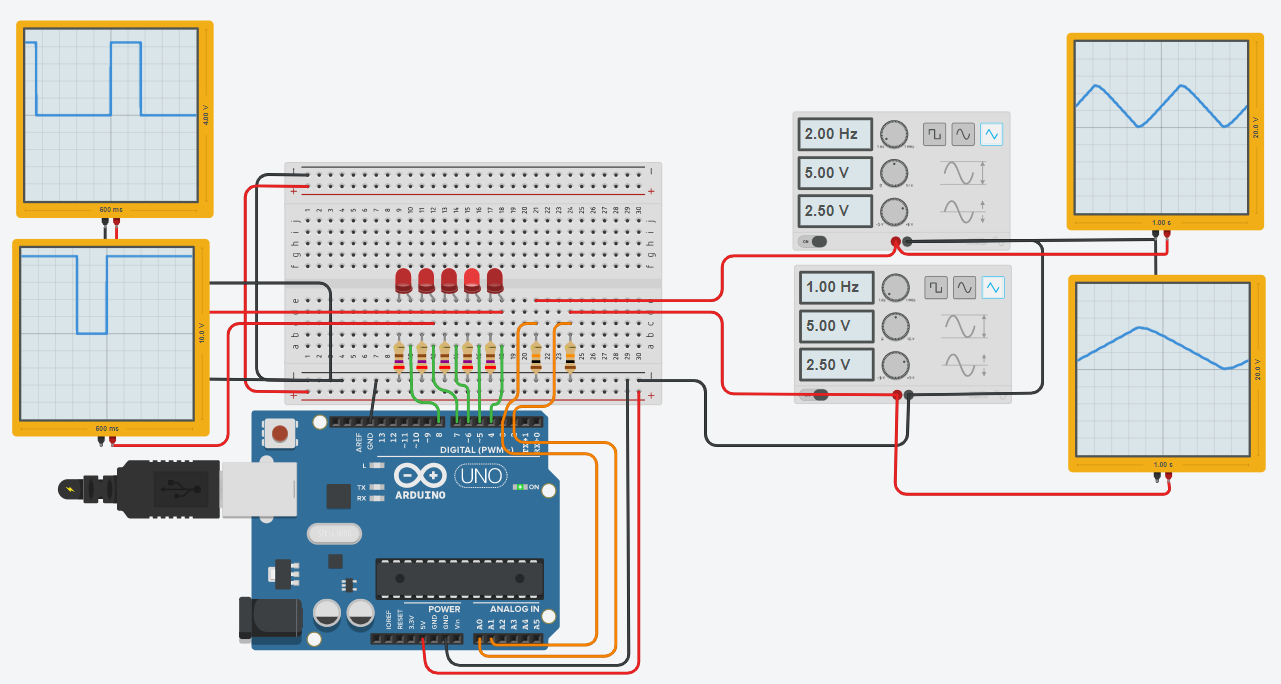
\includegraphics[width=0.8\linewidth]{fig/Fig2.png}
	\caption{Esquema de conexión del Arduino, Generador de funciones y Osciloscopio}
	\label{fig:fig2}
\end{figure}


El código del Anexo B implementa las funciones lógicas AND, OR. Un repaso de como implementar funciones en C se muestra en \href{https://aprendiendoarduino.wordpress.com/2016/11/16/funciones-definidas-por-usuario-2/}{este enlace.} 

\subsubsection{Conteste las preguntas:}

Guarde los datos del puerto serial en un archivo .TXT e importelos en MS EXCEL para graficar los datos.
Se recomienda utilizar el monitor serial de MS CODE STUDIO dado que este permite salvar los datos.
¿Se logra apreciar las señales triangulares y digitales?
¿Las gráficas de las señales digitales de entrada y salida cumplen las tablas de verdad de las conectivas lógicas?
¿Cual es el voltaje de entrada en bajo máximo $V_{IL} max$?,
¿Cual es el voltaje de entrada en alto mínimo $V_{IH} min$?,
¿Cual es el error que presenta las mediciones de los voltajes ?,
¿Si desea un error de $\pm1$ mV, de cuantos bits debe ser el ADC?¿Explique?
%\chapter{Programación de funciones combinacionales.}

\section{Objetivos}
Este es un laboratorio introductorio que busca:
\begin{itemize}
	{\small
	 \item  Programar funciones booleanas combinacionales en Arduino.
	 \item  Verificar la compuertas NAND y NOR son en si mismas un conjunto Universal, equivalentes a el conjunto de conectivas lógicas OR, AND y NOT.
	\item  	Verificar que a partir de los mintérminos de una expresión lógica se obtienen los circuitos con compuertas NAND y de los maxtérminos, los circuitos con compuertas NOR.
	\item  Verificar que para obtener la solución mínima de un circuito lógico, es necesario sintetizar los circuitos tanto por mintérminos como por maxtérminos. 
	\item Programar multiplexores $4\times1$, $8\times1$.
	\item Programar un DECOdificador Binario a Decimal.
 }
\end{itemize} 


\section{Equipos y materiales}
Para este laboratorio de necesitaran:
\begin{itemize} 
	{\small \item 1 Arduino UNO o equivalente: MEGA o ESP32.
	\item 1 Multímetro.
	\item 10 Resistencias de 270 o 330 $\Omega$.
	\item 5 Resistencias de 1k$\Omega$.
	\item 10 interruptores pulsadores.
	\item 1 Protoboard.
	\item 10 Diodes emisor de luz (LEDs).
	\item 1 Computadora portátil.}
\end{itemize}

\section{Marco de referencia}

Un circuito combinacional digital es un circuito que produce una o varias salidas en función de sus entradas actuales. Es decir, no mantiene ningún estado interno y su salida depende exclusivamente de sus entradas en el momento actual.
Existen muchas formas de implementar circuitos combinacionales, a partir de contactos eléctricos, válvulas neumáticas, transistores, software, etc. Sin embargo cualquier circuito lógico combinacional se puede expresar mediante cuatro formas equivalentes que describen su funcionamiento: ecuación lógica, tabla de verdad, diagrama de tiempo, y circuito eléctrico. 
Puede encontrar información adicional en el siguiente enlace \href{https://es.wikipedia.org/wiki/Sistema_combinacional}{https://es.wikipedia.org/wiki/Sistema\_combinacional}.   

\subsection{Implementan de expresiones Booleanas }

Un circuito combinacional  puede ser representado de distintas formas, pero la más común es mediante una ecuación lógica, por ejemplo: 
\begin{equation}
\label{Ec1}
F(a,b,c)=ab+\bar{a}\bar{b}c
\end{equation}

La expresión anterior posee una representación en suma de productos (SDP), puede ser implementada en C de la siguiente forma:

		 \begin{lstlisting}[language=Arduino,numbers=none, showstringspaces=false]
		bool F(bool a,bool b,bool c){
			return  a&&b||!a&&!b&&c;
		}
		\end{lstlisting} 

Existen ocho formas estándar de implementar la ecuación \eqref{Ec1} digital-mente y por consecuencia en software . Otras maneras de implementar las funciones lógicas  son con el producto de sumas (PDS), las implementaciones a dos niveles  NAND/NAND y NOR/NOR, todas las implementaciones deben arrojar los mismos resultados.

Por otra parte, la ecuación \eqref{Ec1} es equivalente a la expresión booleana  NAND/NAND si se niega dos veces y se aplica el \href{https://es.wikipedia.org/wiki/Leyes_de_De_Morgan}{Teorema de Morgan}.


\begin{eqnarray}
\label{Ec2}
F(a,b,c)=ab+\bar{a}\bar{b}c \\
F(a,b,c)=\overline{\overline{ab+\bar{a}\bar{b}c }} \\  \label{Ec3}
F(a,b,c)=\overline{\overline{ab}\cdot\overline{\bar{a}\bar{b}c}}
\end{eqnarray}


Notece que la ecuacion \eqref{Ec3} necesita conectivas lógicas (funciones) de 2 y 3 entradas. Esto no es un problema cuando se implementa en SOFTWARE, pero sí se requiere hacer una implementación fisica hay que aplicar el Algebra Booleana para dejar la expresión en términos de conectivas de solamente dos entradas. Lo que se hace es que el término de tres literales, le aplicamos una doble negación tal como sigue.

\begin{eqnarray}
\label{Ec5}
F(a,b,c)=\overline{\overline{ab}\cdot\overline{\overline{\overline{\bar{a}\bar{b}}}\cdot c}} 
\end{eqnarray}

La expresión \eqref{Ec5} se encuentra en términos de conectivas NAND de dos entradas y se puede implementar en ARDUINO  de la siguiente forma:
{\footnotesize 
\begin{lstlisting}[language=Arduino,numbers=none, showstringspaces=false]
bool F(bool a, bool b, bool c){
	bool resul = false;
	resul = NAND(NAND(a,b),NAND(NAND(NAND(NAND(a,true),NAND(b,true)),true),c));
	return resul;
}
\end{lstlisting} 
}
donde la NAND de dos entradas es:

		\begin{lstlisting}[language=Arduino,numbers=none, showstringspaces=false]
		bool NAND(bool x, bool y){
			return !(x && y);
		}
		\end{lstlisting}

\subsection{Multiplexores y Decodificadores}

Un \href{https://es.wikipedia.org/wiki/Multiplexor}{multiplexor} (Mux) es un circuito combinacional con $2^{n}$ entrada, más $n$  entradas selectoras o de control y una salida. Este circuito combinacional selecciona con las $n$ entradas control,  el valor booleano de una entrada entre $\left[ 0,2^{n}-1\right]$ y coloca dicho valor en la salida. La ecuación general de cualquier multiplexor es la siguiente,

\begin{equation}
MUX=\sum_{i=0}^{2^{n}-1} I_{i}\cdot \mathbb{S}_i
\end{equation}
donde $\mathbb{S}_i$  es la $i$-ésima permutacion de las entradas de selección. A modo de ejemplo un Mux $2 \times 1$
 posee dos entradas digitales y una de control y una salida. Un Mux $4 \times 1$ posee cuatro entradas digitales más dos de control y una salida, Un Mux $8 \times 1$ posee ocho entradas digitales más tres de control y una salida.
 
La ecuación de un Mux $4 \times 1$ es la siguiente,

\begin{equation}
	F(I_0,I_1,I_2,I_3,S_0,S_1)=I_0\bar{S_1}\bar{S_0}+I_1\bar{S_1}S_0+I_2S_1\bar{S_0}+I_3S_1S_0  \;\; .
\end{equation} El código para implementar dicho multiplexor es similar al siguiente,
{\footnotesize 
\begin{lstlisting}[language=Arduino,numbers=none, showstringspaces=false]
bool F(bool I0,bool I1,bool I2,bool I3,bool S1,bool S0){
	return (I0&&!S1&&!S0 || I1&&!S1&&S0 || I1&&S1&&!S0 || I3&&S1&&S0) ;
}
\end{lstlisting}
}
Los circuitos que realizan función inversa del multiplexor se  llama \href{https://es.wikipedia.org/wiki/Demultiplexor}{Demultiplexores}  y usualmente tiene una entrada digital más $n$ entradas de selección y $2^{n}$ salidas digitales.

Otro ejemplo de circuito combinacional son los \href{URL}{Decodificadores} y \href{https://es.wikipedia.org/wiki/Codificador}{Codificadores}.  Un codificador es un circuito combinacional con $2^{n}$ entradas y $n$ salidas, cuya misión es presentar en la salida el código binario correspondiente a la entrada activada. Mientras que un decodificador hace el trabajo inverso, recibe un código binario y lo transforma en cualquier otro código, ya sea  binarios como el Gray o exceso 3; o otras reprentaciones numericas: octal, decimal, hexagecimal. La figura \ref{fig:decoderexample} muestra la implementan digital de un decodificador de 2 a 4 líneas, la tabla de verdad del circuito y las ecuaciones características de cada salida. 
\begin{figure}
	\centering
	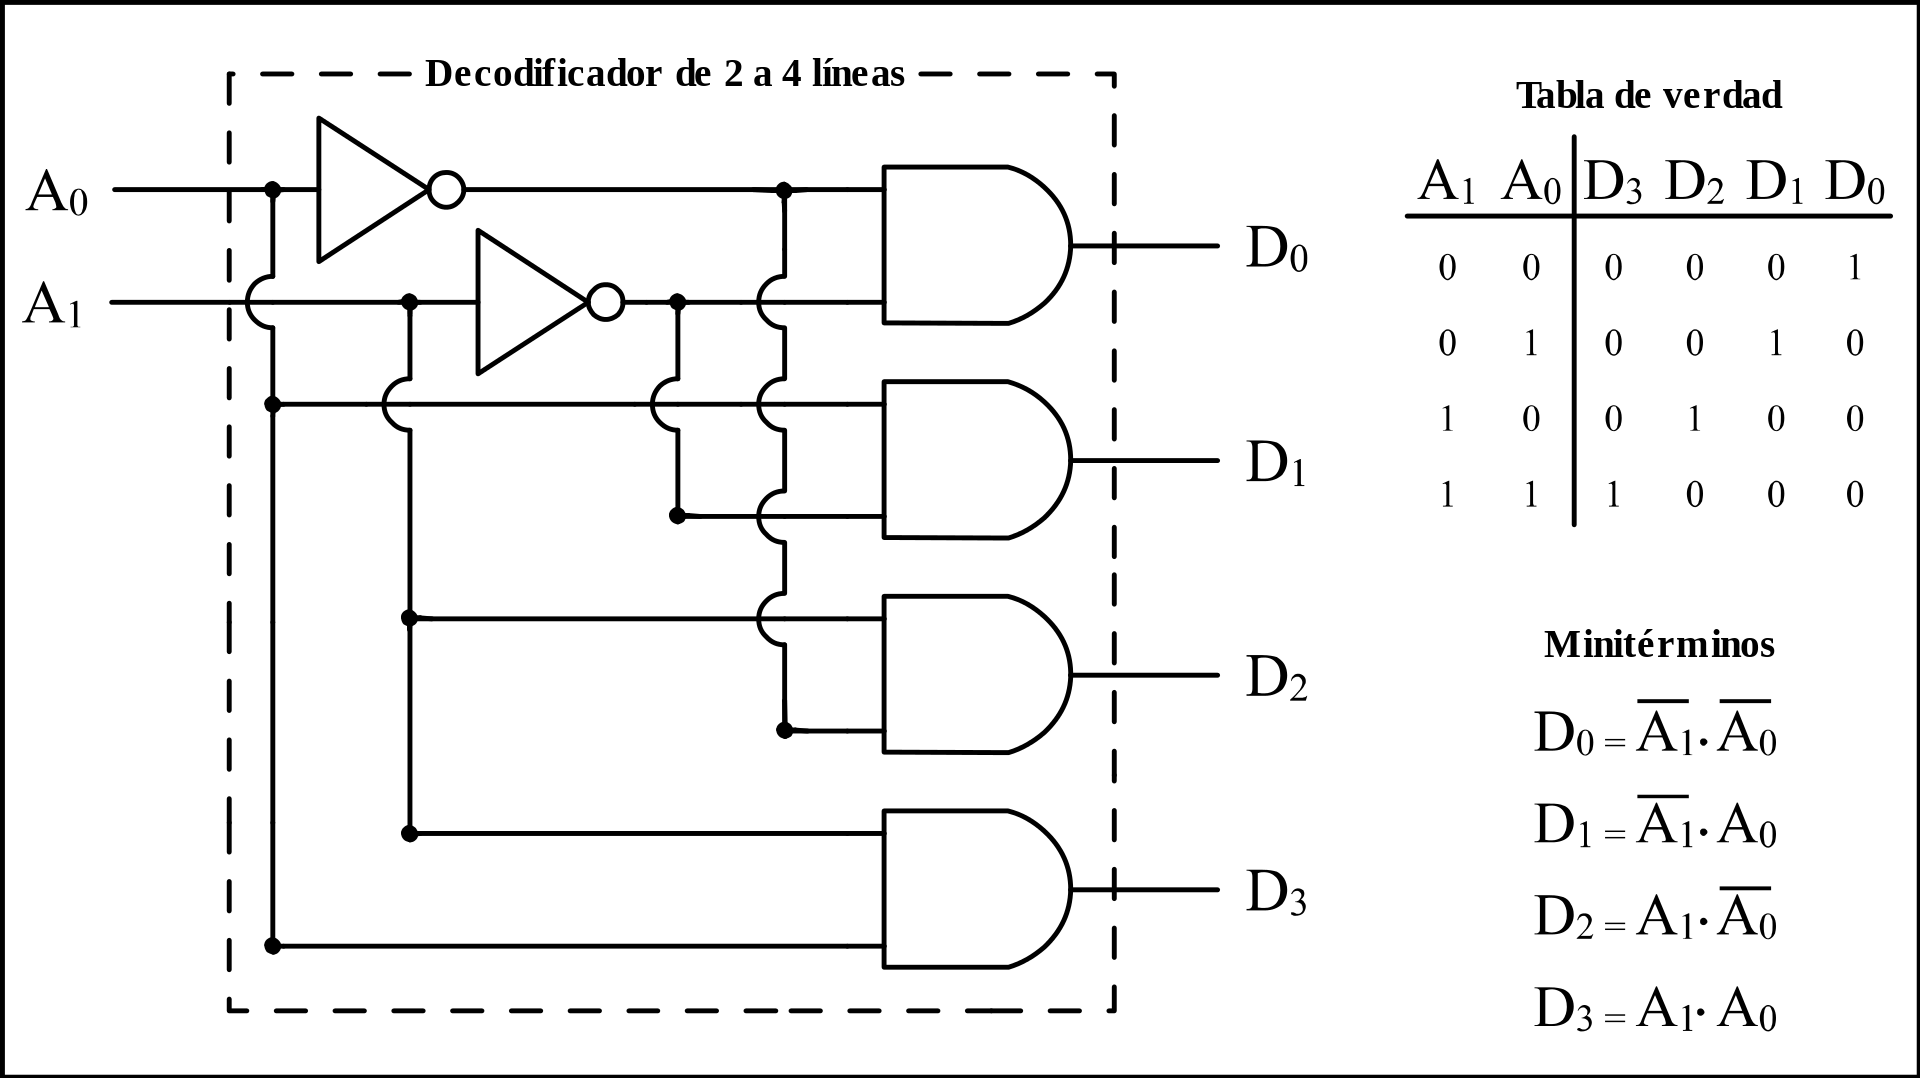
\includegraphics[width=0.7\linewidth]{fig/Decoder_Example.png}
	\caption{Decodificador de código binario de dos bits a cuatro líneas de salida.  }
	\label{fig:decoderexample}
\end{figure}

Una posible implementación para Arduino de este decodificador es la siguiente.

\begin{lstlisting}[language=Arduino,numbers=none, showstringspaces=false]
	byte  DECO (bool A0, bool A1)
	{
		int i=0;
		bool D[4]={false, false, false, false};
		byte deco=0;
	
		D[0]=!A1&&!A0;
		D[1]=!A1&&A0;
		D[2]=A1&&!A0;
		D[3]=A1&&A0;
	
		for (i=0; i<sizeof(D);i++)
		{
			bitWrite(deco, i, D[i]);
		}
	return deco;
	}
\end{lstlisting}
  
\section{Metodología}

Este laboratorio tiene una duración de 4 lecciones, repartidas en dos semanas. Los estudiantes deben mostrar durante las clases programadas las tres actividades propuestas. Deben recabar fotografías y resultados de los equipos de medición para elaborar las evidencias. Las evidencias se subirán al TecDigital la semana siguiente finalizadas las actividades.

\section{Práctica en Clase}

\subsection{Actividad 1}

Programe en Arruino una lógica combinacional que resuelva el siguiente problema.  En una planta industrial se desea automatizar un motor y una alarma de acuerdo a 4 sensores llamados a, b, c, d.  La señal del motor se representa por la función lógica f1, y se validará  cuando el sensor  a y b estén activos, o cuando  este b y  este el sensor d o cuando estén a, c y d. Por otro lado, la señal de  alarma (función f2), se activa siempre que estén todos los sensores apagados excepto a o todos apagados excepto c o  estén c y d encendidos y el resto apagados. También la alarma se encienden cuando todos los sensores son activados o cuando estén todos excepto d o todos excepto c.
 
 En el Arduino los Pines $\left\lbrace 0,1,2,3\right\rbrace $ serán las entradas digitales {a,b,c,d}. Las salidas o respuestas de las funciones se dividen en dos grupos, los pines $\left\lbrace 5,6,7\right\rbrace $ se reservan para f1. Se deben implementar tres funciones:  la suma de productos (SDP), el producto de suma(PDS) y la funcion resuelta por conectivas NAND/NAND.   Por otro lado la función f2  mostrar\'{a} su respuesta mediante los pines 
 $\left\lbrace 8,9,10\right\rbrace $, dicha función es implementada mediante SDP, PDS y conectivas NOR/NOR.
 
 
\subsubsection{Conteste las preguntas:}

¿Cómo sería el circuito digital de cada una de las funciones implementadas?
¿Como es la tabla de verdad experimental de cada salida versus la tabla teórica?


\subsection{Actividad 2}

Programe las funciones de un Multiplexor 2x1, 4x1 y 8x1.
Por otra parte, existe un circuito  combinacional que se comporta como la siguiente tabla de verdad. Cuadro \eqref{tab:tv}.

\begin{table}[H]
\centering
\caption{Comportamiento esperado de la estructura lógica.}
\label{tab:tv}
\begin{tabular}{|c|c|c|}

	\hline 
	a 	& b  & $F(a,b)$  \\ 
	\hline 
 	0	& 0 &  $c + d$\\ 

	0	& 1 &  $\overline{c + d}$\\ 

	1	& 0 &  $\overline{c \cdot d}$\\ 

	1	& 1 &  $c \oplus d$\\ 
	\hline 
\end{tabular} 

\end{table}

\subsubsection{Conteste las preguntas:}

¿El comportamiento de un multiplicador $8 \times 1$ coincide con la tabla teórica?
En la funcion Loop() , llame la función del MUX  $8 \times 1$ e ingrese parámetros $\left\lbrace a,b,c,d \right\rbrace $ de tal forma que se comporte igual que la tabla de verdad presentada en el Cuadro \ref{tab:tv}.¿Tiene el mismo comportamiento?
¿Es posible implementar la T.V. con dos MUX $4 \time 1$ y un MUX  $2 \time 1$?¿Como se implementa?

\subsection{Actividad 3}

Implemente en un Arduino un decodificador de 3 bits a Octal. En otro Arduino programe la función de un codificador Octal a binario de 3 bit. Conecte ambos Arduinos, las entradas del primer arduino se conectan a botoneras, las salidas del primer arduino se conectan con las entradas del segundo Arduino y las salidas del segundo Arduino se conectan a LEDs.  


\subsubsection{Conteste las preguntas:} 
¿La tabla de verdad del codificador es idéntica a la teórica o esperada?
¿La tabla de verdad del decodificador es idéntica a la teórica o esperada?
¿Como es la salida del segundo Arduino respecto a las entradas del primero?

%\chapter{Laboratorio: Programación Flip-flops, Contadores, Drivers.}


\section{Objetivos}
Este es un laboratorio introductorio que busca:
\begin{itemize}
	{\small
	 \item  Programar en ARDUINO el comportamiento de los Flip-Flop J-K, T, D activador por flanco positivo y el Biestable Set-Reset.
	 \item  Estudiar que los Flip-Flop usan reloj para sincronizar los cambios pero los biestables son asincrónicos.
	 \item  Programar en ARDUINO el comportamiento de un Contador ascendente decendente para el control de un parqueo.
	 \item  Programar un driver para un motor unipolar y bipolar con Arduino.
 }
\end{itemize} 


\section{Equipos y materiales}
Para este laboratorio de necesitaran:
\begin{itemize}
	{\small \item 1 Arduino UNO o equivalente: MEGA o ESP32.
	\item 1 Multímetro.
	\item 10 Resistencias de 270 o 330 $\Omega$.
	\item 5 Resistencias de 1k$\Omega$.
	\item 10 interruptores pulsadores.
	\item 1 Protoboard.
	\item 1 display de 16 x 2 segmentos.
	\item 1 motor a pasos bipolar.
	\item 1 chip L293D con dos puentes H para motor bipolar.
	\item 1 motor a pasos unipolar. 
	\item 1 driver 28BYJ-48 para motor unipolar con driver  ULN2003.
	\item 1 Computadora portátil.}
\end{itemize}

\section{Marco de referencia}

 Los sistemas secuenciales tienen la característica que sus salidas en cualquier momento determinado son funciones tanto de las entradas externas en ese momento como de la secuencia de salidas pasadas. Esto quiere decir que esas salidas son memorizadas para usarlas como entrada en el siguiente análisis. El análisis de las entradas y memorias se ejecuta en los flanco positivos o negativos de una señal de control o reloj.
 
 Los dispositivos encargados de memorizar solo son capaces de almacenar información binaria, es decir un cero o uno lógico. Estos elementos de memoria son llamados cerrojos y bi-estables (\textit{latches} y \textit{flip-flops} ) , y la diferencia principal entre estos dos tipos de elementos es que los primeros son asincrónicos, es decir no dependen de una señal de reloj, y los segundos (\textit{flip-flops}) si dependen de un reloj externo. 

Existen varios tipos de cerrojos y bi-estables, pero para efectos del laboratorio se estudiarán el cerrojo Set-Reset, y los bi-estables J-K, D, T. El cerrojo S-R tienen las siguientes ecuaciones características:

\begin{eqnarray}
\label{lab3:Ec1}
Q=S+Q\bar{R} \\ \label{lab3:Ec2}
Q=(S+Q)\bar{R}
\end{eqnarray}
donde $S$ es la entrada que pone un uno lógico en la salida $Q$, por otro lado la entrada $R$ restablece la salida $Q$. La ecuación \eqref{lab3:Ec1} da prioridad a la entrada set, mientras que la ecuación \eqref{lab3:Ec2} da prioridad a la entrada reset. El Cuadro \ref{tab:SR} muestra el comportamiento esperado del cerrojo S-R, si el S-R es con prioridad al Set la X vale un uno lógico, y si es prioridad al reset la X vale un cero lógico. 

\begin{table}
	\centering
	\caption{Tabla de verdad del cerrojo S-R.}
	\label{tab:SR}
	\begin{tabular}{cccc}
		\toprule
		$S$ & $R$ & $Q+$ & $\bar{Q}+$ \\
		\midrule
		0 & 0 &	$Q$	& $Q$ \\ 
		0 & 1 &	0 & 1 \\ 
		1 & 0 &	1 &	0 \\ 
		1 & 1 &	X &	X \\ 	
		\bottomrule
	\end{tabular} 
\end{table} 

Los bi-estables J-K poseen poseen tres entradas: J, K y el reloj Clk. La ecuación característica esta defina por \eqref{lab3:Ec4}, mientras que la tabla de verdad se presenta en el Cuadro \ref{tab:JK}. 

\begin{eqnarray}
	\label{lab3:Ec4}
%%	Q=J\bar{Q}+Q\bar{K} \\ \label{lab3:Ec5}
	Q=(J\bar{Q}+Q\bar{K})\cdot\uparrow CLK
\end{eqnarray}


\begin{table}
    \centering
    \caption{Tabla de verdad del Latch J-K.}
    \label{tab:JK}
    \begin{tabular}{ccccc}
        \toprule
        $J$ & $K$ & $CLK$ & $Q+$ & $\bar{Q}+$ \\
        \midrule
        X & X &	X &	$Q$	& $\bar{Q}$	\\ 
        0 & 0 &	$\uparrow$ & $Q$ & $\bar{Q}$ \\ 
        0 & 1 &	$\uparrow$ & 0 & 1 \\ 
        1 & 0 & $\uparrow$ & 1 & 0 \\ 	
        1 & 1 &	$\uparrow$ & $\bar{Q}$ &  $Q$ \\ 	
        \bottomrule
    \end{tabular} 
\end{table} 

Por otra parte los bi-estable tipo de D y T son casos particulares del bi-estable J-K y sus ecuaciones características estan definas por \eqref{lab3:Ec6} y \eqref{lab3:Ec7}. 

\begin{eqnarray}
\label{lab3:Ec6}
Q=D\cdot\uparrow CLK \\ \label{lab3:Ec7}
Q=(T\bar{Q}+Q\bar{T})\cdot\uparrow CLK
\end{eqnarray}


\subsection{Implementación de Cerrojos y Biestables}

La implementación de cerrojos y bi-estables dependen de como se llamen las funciones características de los elementos de memoria. Para los cerrojos se llaman en la rutina principal y los biestables se llaman dentro de un rutina de interrupción por hardware.

El \textit{latch Set-Reset} con prioridad al reset es una función que se implementa en la sección de funciones de la siguiente forma,

		 \begin{lstlisting}[language=Arduino,numbers=none, showstringspaces=false]
		bool RS(bool S,bool R,bool Q){
			return  (S||Q)&&!R;
		}
		\end{lstlisting} donde $S$ y $R$ son entradas digitales y $Q$ es una variable global del tipo booleano. Al no de pender de una señal de reloj, esta función se llama dentro del rutina principal \textbf{loop()}.

Por otra parte, los \textit{flip-flop} funcionan si existe un flanco positivo o negativo de reloj, para emular este comportamiento se usa  la interrupción por \textit{hardware}, pin 2 o 3  en un Arduino UNO. La interrupción por hardawre se habilita dentro de la sección \textbf{setup()}, con el comando \href{https://reference.arduino.cc/reference/en/language/functions/external-interrupts/attachinterrupt/}{ \textbf{attachInterrupt()}}.

	\begin{lstlisting}[language=Arduino,numbers=none, showstringspaces=false]

void setup(){
// Initializa los pines:
	{
		//Linas de código
	}	
	/* Habilita la Rutina de Interrpcion por Hardware (RIH) en
	cada flanco positivo que se detecta en PIN #2 */
	
	attachInterrupt(digitalPinToInterrupt(2), RIH, RISING);
}
\end{lstlisting}

La rutina de interrupción detiene la rutina principal \textbf{loop()} y ejecuta una rutina definida por el usuario llamada en este caso RIH. Esta rutina no posee parametros de entrada, ni de salida. Dentro de la rutina  RIH si se puede llamar a otras funciones programadas, por ejemplo se llama la función del bi-estable J-K definida en la sección de funciones. 


		\begin{lstlisting}[language=Arduino,numbers=none, showstringspaces=false]
		
		bool JK(bool J, bool K, bool Q){
			return (J&&!Q)||(!K&&Q);
		}
		\end{lstlisting}

\subsection{Contadores y Secuenciadores}


El diseño digital de contadores, secuenciadores como por ejemplo la lógica de control parar motores a pasos (\textit{drivers}) se simplifica con un lenguaje de alto nivel como C/C++, por lo tanto no es necesario implementar como si fuera un diseño digital, en cambio usaremos funciones y estructuras de control. Por ejemplo un contador ascendente/descendente de 0-20 se puede programar de forma similar a función \textbf{Contador()}.
\begin{lstlisting}[language=Arduino,numbers=none, showstringspaces=false]
int Contador (bool Sube, bool Baja, int Valor){
	if (Sube && (Valor <20)){
		Valor++;
	}
	if(Baja && (Valor >0)){
		Valor--;
	}
	return Valor;
}
\end{lstlisting}
 
De manera similar un secuenciador de cuatro etapas que genere la secuencia $\{1100_{2}, 0110_{2}, 0011_{2}, 1001_{2}\}$ o su equivalente en decimal    $\{12,6,3,9\}$, puede servir para controlar los relays o transistores de un \href{https://es.wikipedia.org/wiki/Motor_paso_a_paso}{motor a pasos}. La función para controlar un motor a pasos unipolar es similar a la siguiente:


\begin{lstlisting}[language=Arduino,numbers=none, showstringspaces=false]

byte Driver(int Paso){
	byte output = 0;
	if(Paso==1){
		output=0b00001100; 
	}
	if(Paso==2){
		output=0b00000110;
	}
	if(Paso==3){
		output=0b00000011;
	}
	if(Paso>=4){
		output=0b00001001;
	}
	return output;
}
\end{lstlisting} donde el parámetro de entrada (Paso), es el resultado dado por un una función que cuenta entre {1-4}. Si el resultado del la función \textbf{Driver()} se desea imprimir a los pines digitales, esto se realiza con la función \href{https://www.arduino.cc/reference/en/language/functions/bits-and-bytes/bitread/}{\textbf{bitRead()}} .
  
\section{Metodología}

Este laboratorio tiene una duración de 4 lecciones, repartidas en dos semanas. Los estudiantes deben mostrar durante las clases programadas las tres actividades propuestas. Deben recabar fotografías y resultados de los equipos de medición para elaborar las evidencias. Las evidencias se subirán al TecDigital la semana siguiente finalizadas las actividades.

\section{Práctica en Clase}

\subsection{Actividad 1}

Programe un Arduino Uno con el comportamiento de un Latch Set-Reset prioridad al set, y los flip-flops J-K, T, D.  Por el pin 2 entra una señal de reloj con frecuencia ajustable entre 5Hz y 1kHz. El Pin 3  se conecta a una botonera y representar\'a las  S, J, D y T.  El pin 4 se conecta a otra botonera y se  reserva para la entrada R y K. La salida del cerrojo S-R se muestra mediante a un LED conectado al PIN 4. El Pin 5 se conecta a otro LED y será la salida del Bi-estable J-K. Los pines 6 y 7, son las salidas de los flip-flops T y D y también se conectan a LEDs. Imprima los resultados en el puerto serial, ajuste la velocidad del puerto con valores de: \{ 9600, 14400, 19200, 28800, 38400, 57600\}bps según la frecuencia del reloj.
 
\subsubsection{Conteste las preguntas}

¿Es el comportamiento programado es idéntico a la tablas de verdad teóricas o existen diferencias? Explique.
¿Cual es la diferencia práctica entre un S-R y un J-K? ¿Cual responde más rápido?,
¿Que pasa si el reloj posee una frecuencia de 1KHz, son las respuestas distintas o iguales? Explique. 
¿Como son las gráficas obtenidas si los datos se gráficas en Excel?

\subsection{Actividad 2}

Se desea automatizar un paqueo automotriz que posee exactamente 20 campos disponibles. El parqueo tiene una entrada y una salida como se aprecia en la Figura \ref{fig:parqueo}. 

Tanto la entrada como la salida posee sensores de proximidad (usted usará 2 botones pulsadores para emular  esto). Además el Arduino controlará las 2 agujas de acceso (2 LEDs). Cuando un automóvil ingrese al parqueo, se abrirá la aguja (LED) si y solo si hay cupo disponible, sino el LCD parpadeará el número cero. Si se abre la aguja usted debe mostrar en la pantalla del LCD cuando cupos quedan disponibles. Por otra parte cuando sale un carro también se incrementa en uno los campos disponibles y se muestra en el LCD.

Cuando se abre cualquier aguja, el LED que lo representa, debe permanecer encendido por 5 segundos y luego se apagará.

El Display posee una estructura de 16 x 2 caracteres, en el primer reglón colocarán el contador de cupos disponibles como se aprecia en la figura \ref{fig:dislay}. En el segundo reglón aparecerá durante el tiempo que LED  este encendido las palabras ENTRADA $>$ o SALIDA $<$  respectivamente. Recuerde que un vehículo puede ingresar mientras otro esta saliendo y viceversa.

\begin{figure}
	\centering
	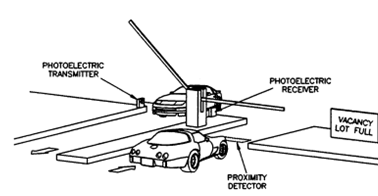
\includegraphics[width=0.7\linewidth]{fig/Parqueo.png}
	\caption{Entrada y salida del parqueo.}
	\label{fig:parqueo}
\end{figure}

\begin{figure}
	\centering
	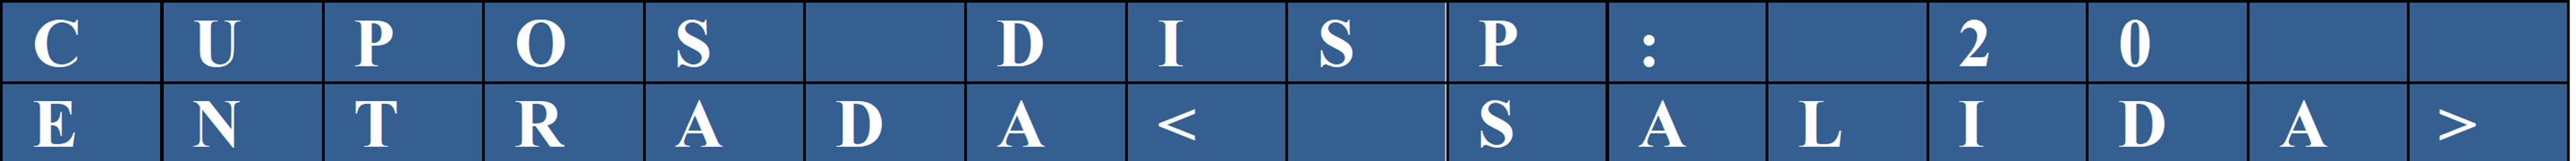
\includegraphics[width=0.7\linewidth]{fig/Dislay.png}
	\caption{Display de 16 x 2 caracteres.}
	\label{fig:dislay}
\end{figure}

Para realizar esta actividad debe estudiar los siguiente:
 Estudiar la \href{https://docs.arduino.cc/software/ide-v1/tutorials/installing-libraries#.Uyd116h5PRk}{instalación de librerías} en Arduino. En Arduino existen mas de cuatro mil librerías que pueden ser consultadas en este \href{https://www.arduino.cc/reference/en/libraries/}{enlace}.
 Estudiar el uso de un display 16x2 caracteres usando la librería \href{http://arduino.cc/en/Tutorial/LiquidCrystalDisplay#.UyPQYfl5OSo }{\textbf{LiquidCrystal.h}}.
 Estudiar la librerías \href{https://github.com/sstaub/Timer}{\textbf{Timer.h }}, \href{https://github.com/kiryanenko/SimpleTimer}{\textbf{SimpleTimer.h}} para la generación de pulsos controlados.
 
\subsubsection{Conteste las preguntas:}

¿Que pasa si ambos botones, entrada y salida, se presionan de forma simultanea?
¿Puede realizar un experimento completo donde se muestre como se llena y vacía el parqueo y exportar los resultados al puerto serial?

% \subsection{Actividad 3}

% Realice un programa en Arduino que controle dos motores a pasos, con un botón conectado al Pin 1 los dos motores arrancan o paran. Si se arranca los motores, en pantalla se mostrará la palabra RUN, y el sentido de giro  de giro derecho ($>>$).
% \begin{figure}[h]
% 	\centering
% 	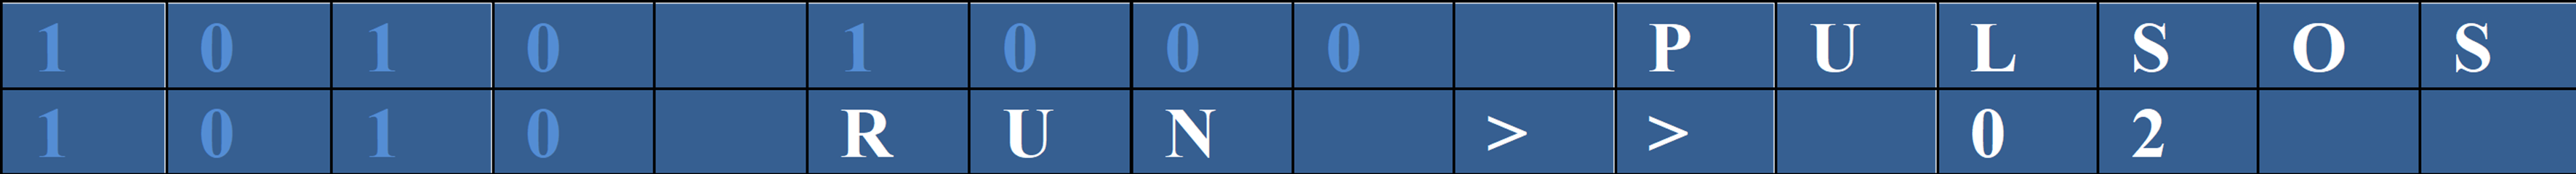
\includegraphics[width=0.7\linewidth]{fig/Fig3.png}
% 	\caption{Display 16X2 caracteres.}
% 	\label{fig:fig3}
% \end{figure}
% Si se presiona el nuevamene Pin 1 (pare), los motores se detienen indicando la palabra STOP en el Display de cristal liquido (LCD).
% \begin{figure}[H]
% 	\centering
% 	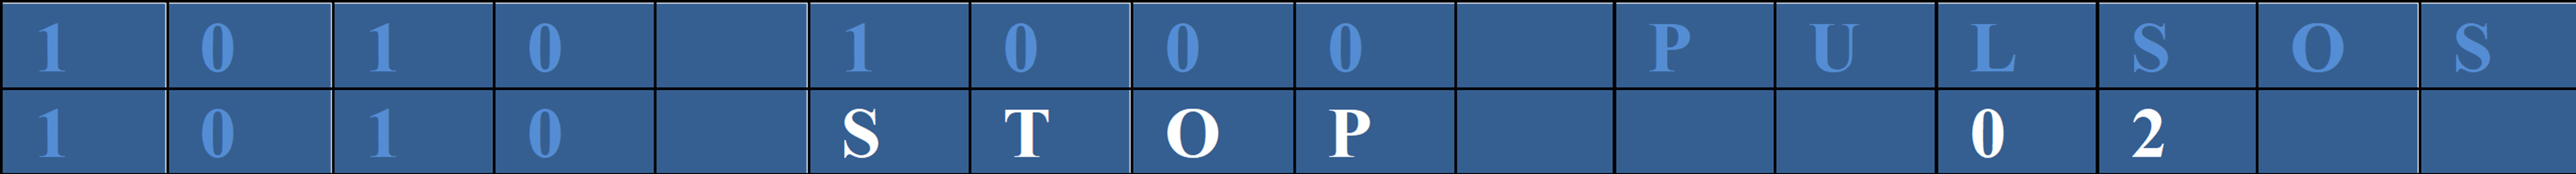
\includegraphics[width=0.7\linewidth]{fig/Fig4.png}
% 	\caption{Información mostrada en Display cuando se presiona el boton de parada.}
% 	\label{fig:fig4}
% \end{figure}

% Si presiona el botón conectado al PIN (3) en la pantalla los dos motores cambiaran de sentido de giro, y en pantalla aparecerá ($<<$). Si se presiona nuevamente el botón conectado al Pin (2), los motores cambiaran de sentido nuevamente y en pantalla aparecerá ($>>$).

% Si se presionan botones UP o DOWN (Pines 4 o 5) la velocidad de pulsos por segundo se incrementará ($\uparrow$) o se excrementará ($\downarrow$) de uno en uno, desde 2 p/sec hasta 40p/sec. En pantalla se montará las siguientes flechas.
% \begin{figure}[H]
% 	\centering
% 	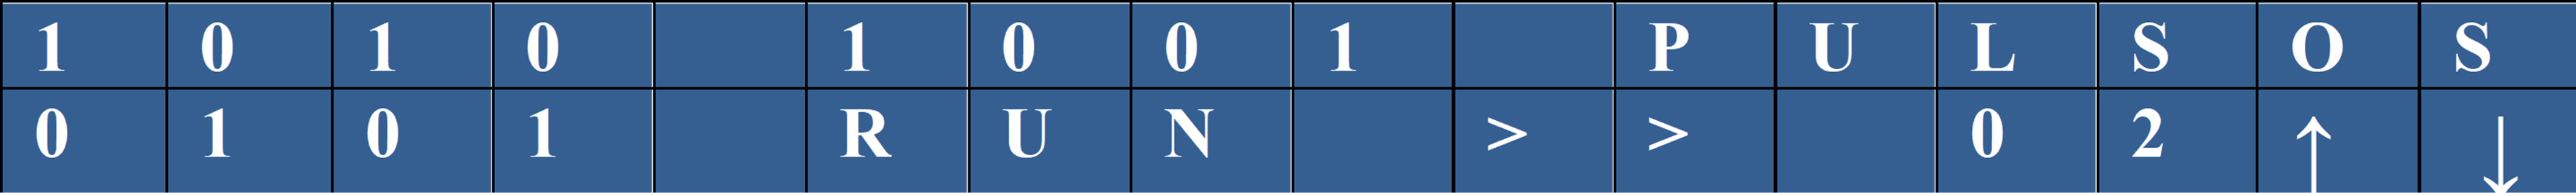
\includegraphics[width=0.7\linewidth]{fig/Fig5}
% 	\caption{Flechas mostradas en Display cuando se modifican los pulsos. }
% 	\label{fig:fig5}
% \end{figure}
% Los motores unipolares se controlan con las señales S1, S2, S3, S4 que se muestran en el Display. Los motores Bipolar necesitan dos puentes H y cada puente tendrá las señales de control Q1, Q2, Q3, Q4.  Las señales de control Sx y Qx tendrán valores de 1 o 0 únicamente.

% \begin{figure}[H]
% 	\centering
% 	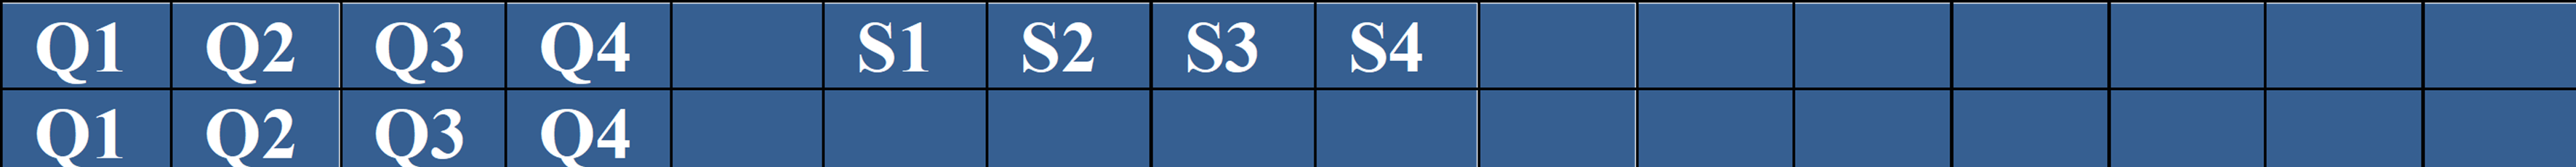
\includegraphics[width=0.7\linewidth]{fig/Fig6}
% 	\caption{Señales de control para los motores.}
% 	\label{fig:fig6}
% \end{figure}

% El circuito de potencia de un puente H se aprecia en la figura \ref{fig:puenteh}.
% \begin{figure}[H]
% 	\centering
% 	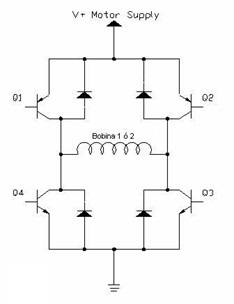
\includegraphics[width=0.4\linewidth]{fig/PuenteH}
% 	\caption{Puente H para un motor Bipolar.}
% 	\label{fig:puenteh}
% \end{figure}

% Conecte un motor Unipolar o bipolar con el circuito de potencia al Arduino. Utilize el circuito de potencia adecuado según su motor. Ponga en el Eje cinta para ver el sentido de jiro.

% \subsubsection{Conteste las preguntas:} 

% ¿Puede mostrar las tablas de excitación generadas por el arduino para controlar los motores?
% ¿Son estas tablas similares a la teóricas?

%----------------------------------------------------------------------------------------
%	APPENDIX
%----------------------------------------------------------------------------------------

\appendix
\chapter{Repositorio de código}
\label{ap:osc}
\section{Código para sección \ref{l2:a1}}
\label{ApendiceA}

{\scriptsize 
    \begin{lstlisting}[language=Arduino,numbers=none, showstringspaces=false]
    /*
      ASCII table
    
      Prints out byte values in all possible formats:
      - as raw binary values
      - as ASCII-encoded decimal, hex, octal, and binary values
    
      For more on ASCII, see http://www.asciitable.com and http://en.wikipedia.org/wiki/ASCII
    
      The circuit: No external hardware needed.
    
      created 2006
      by Nicholas Zambetti <http://www.zambetti.com>
      modified 9 Apr 2012
      by Tom Igoe
    
      This example code is in the public domain.
    
      https://www.arduino.cc/en/Tutorial/BuiltInExamples/ASCIITable
    */
    
    void setup() {
      //Initialize serial and wait for port to open:
      Serial.begin(9600);
      while (!Serial) {
        ;  // wait for serial port to connect. Needed for native USB port only
      }
    
      // prints title with ending line break
      Serial.println("ASCII Table ~ Character Map");
    }
    
    // first visible ASCIIcharacter '!' is number 33:
    int thisByte = 33;
    // you can also write ASCII characters in single quotes.
    // for example, '!' is the same as 33, so you could also use this:
    // int thisByte = '!';
    
    void loop() {
      // prints value unaltered, i.e. the raw binary version of the byte.
      // The Serial Monitor interprets all bytes as ASCII, so 33, the first number,
      // will show up as '!'
      Serial.write(thisByte);
    
      Serial.print(", dec: ");
      // prints value as string as an ASCII-encoded decimal (base 10).
      // Decimal is the default format for Serial.print() and Serial.println(),
      // so no modifier is needed:
      Serial.print(thisByte);
      // But you can declare the modifier for decimal if you want to.
      // this also works if you uncomment it:
    
      // Serial.print(thisByte, DEC);
    
    
      Serial.print(", hex: ");
      // prints value as string in hexadecimal (base 16):
      Serial.print(thisByte, HEX);
    
      Serial.print(", oct: ");
      // prints value as string in octal (base 8);
      Serial.print(thisByte, OCT);
    
      Serial.print(", bin: ");
      // prints value as string in binary (base 2) also prints ending line break:
      Serial.println(thisByte, BIN);
    
      // if printed last visible character '~' or 126, stop:
      if (thisByte == 126) {  // you could also use if (thisByte == '~') {
        // This loop loops forever and does nothing
        while (true) {
          continue;
        }
      }
      // go on to the next character
      thisByte++;
    }
    \end{lstlisting}
}



\section{Código actividad 2}
\label{ApendiceB}
{\scriptsize 
    \begin{lstlisting}[language=Arduino,numbers=none, showstringspaces=false]
    /*
    Instituto Tecnológico de Costa Rica
    LAB #1 de Laboratorio de Control Eléctrico.
    Fecha: 25/01/2023
    Ing. Luis D. Murillo
    
    Este programa apaga el LED cuando se presiona el botón. 
    
    */
    // Declaracione de entradas y salidas
    const int BUTTON =2;  // Boton conectado al pin 2
    const int LED =4;     // LED conectado al pin 4
    
    // CONFIGURACION DE ENTRADAS Y SALIDAS
    void setup() {
        pinMode(LED, OUTPUT);    // configuramos el pin del LED como salida
        digitalWrite(LED, HIGH);  // Encendemos el LED
        pinMode(BUTTON, INPUT);  // configuramos el pin del botón como entrada
    }
    // PROGRAMA PRINCIPAL
    void loop() {
        bool buttonState = digitalRead(BUTTON);  // leemos el estado del botón
        if (buttonState == HIGH) {
            digitalWrite(LED, LOW);  // apagamos el LED
        } else {
            digitalWrite(LED, HIGH);   // encendemos el LED
        }
    }
    \end{lstlisting}
}	


\section{Código actividad 3}

{\scriptsize 
		
	\begin{lstlisting}[language=Arduino,numbers=none, showstringspaces=false]
		 /*
		Instituto Tecnológico de Costa Rica
		Laboratorio de Control Eléctrico.
		Lab #1: Conectiva logicas y señal analógica
		Fecha: 24/01/2023
		Ing. Luis D. Murillo
		
		Implementación de Funciones Lógicas AND, OR, XOR, NAND, NOR de 2 entradas
		*/
		// Declaracione de constantes
			const int PinEntrada[2]={2,3};
			const int PinSalidas[5]={4,5,6,7,8};
			const int PinAnalogico[2] = {A0, A1};
			int ValorAnalojLeido[2]={0,0};
			float ValorVoltage[2]={0.0,0.0};
			boolean Mapa_entradas[2];
			boolean ResultadoLogico[5]={false, false, false, false, false};
		
		// Configuracion de Pines de entrada y salida
		void setup(){
			Serial.begin(9600);
			Serial.println("-----");
			Serial.println((sizeof(PinEntrada)/2));
			Serial.println((sizeof(PinSalidas)/2));
			Serial.println("-----");
		
		// Initializa los pines:
		for (int i = 0; i < (sizeof(PinSalidas)/2); i++) {
			if (i<(sizeof(PinEntrada)/2)) {
				pinMode( PinEntrada[i], INPUT);
			}
			pinMode(PinSalidas[i], OUTPUT);
			}
		delay(2);
		}
		
		void loop()
		{		
			//LECTURA DE LAS ENTRADAS Y SALIDAS 	
			for(int i=0; i<(sizeof(PinSalidas)/2);i++){
				if(i<(sizeof(PinEntrada)/2)){
					// Lectura de entradas digitales
					Mapa_entradas[i]=digitalRead(PinEntrada[i]);
					// Lectura de los valores analógicos
					ValorAnalojLeido[i] = analogRead(PinAnalogico[i]);
					// Funcion de mapeo :
				ValorVoltage[i]= (map(ValorAnalojLeido[i], 0, 1023, 0, 500)/100.0);
				}
			// Escritura de salida digital
			digitalWrite(PinSalidas[i],ResultadoLogico[i]);
			}
		
		//EJECUCION DEL PROGRAMA
			ResultadoLogico[0]=AND(Mapa_entradas[1],Mapa_entradas[0]);
			ResultadoLogico[1]=OR(Mapa_entradas[1],Mapa_entradas[0]);
			ResultadoLogico[2]=XOR(Mapa_entradas[1],Mapa_entradas[0]);
			ResultadoLogico[3]=NAND(Mapa_entradas[1],Mapa_entradas[0]);
			ResultadoLogico[4]=NOR(Mapa_entradas[1],Mapa_entradas[0]);
		
		//IMPRESION DE RESULTADOS ENTRADA Y SALIDAS
		
			Serial.print(Mapa_entradas[0]);
			Serial.print(", ");
			Serial.print(ValorVoltage[0]);
			Serial.print(", ");
			Serial.print(Mapa_entradas[1]);
			Serial.print(", ");
			Serial.print(ValorVoltage[1]);
			Serial.print(", ");
			Serial.println(ResultadoLogico[0]);
			Serial.print(", ");
			Serial.print(ResultadoLogico[1]);
			Serial.print(", ");
			Serial.print(ResultadoLogico[2]);
			Serial.print(", ");
			Serial.print(ResultadoLogico[3]);
			Serial.print(", ");
			Serial.println(ResultadoLogico[4]);
		}
		
		//DEFINICION DE LAS FUNCIONES LÓGICAS
		// Forma de programacion Booleana
		bool AND (bool X, bool Y ){
		return (X && Y ); 
		}
		
		// Forma de programacion con estructuras de control
		bool OR (boolean X, bool Y ){
		if (X || Y) {return true;} 
		else {return false;}
		}
		
		// Completar código
		bool XOR (bool X, bool Y ){
				; 
		}
		
		bool NAND (bool X, bool Y ){
				; 
		}		
		
		bool NOR (bool X, bool Y ){
				; 
		}
		\end{lstlisting}
}

%----------------------------------------------------------------------------------------
%	BIBLIOGRAPHY
%----------------------------------------------------------------------------------------

\bibliographystyle{ieeetr}

\bibliography{referencias}

%----------------------------------------------------------------------------------------


\end{document}